\documentclass{article} % For LaTeX2e

\usepackage{nips12submit_e,times}
\usepackage{pslatex}
\usepackage{amsmath}
\usepackage{amsfonts}
\usepackage{latexsym}
\usepackage{amssymb}
\usepackage{graphicx}
\usepackage{xspace}
\usepackage{multirow}
\usepackage{array}
\usepackage{caption}
\usepackage{subcaption}
\usepackage[numbers]{natbib}

\title{Supplementary Information:\\ Halo, Hyperbole, and the Pragmatic \\ Interpretation of Numbers}
 
\author{
Jean Y. Wu \\
Symbolic Systems Program\\
Stanford University\\
Stanford, CA 94305 \\
\texttt{jeaneis@stanford.edu} \\
\And
Justine T. Kao \\
Department of Psychology\\
Stanford University \\
Stanford, CA 94305 \\
\texttt{justinek@stanford.edu} \\
\AND
Leon Bergen \\
Department of Brain and Cognitive Sciences\\
Massachusetts Institute of Technology \\
Cambridge, MA 02138\\
\texttt{bergen@mit.edu} \\
\And
Noah D. Goodman \\
Department of Psychology\\
Stanford University \\ 
Stanford, CA 94305\\
\texttt{ngoodman@stanford.edu} \\
}

\nipsfinalcopy
\begin{document}

\maketitle

\section{Experiment Scenarios}

% textbooks
\begin{table}[h]
\begin{tabular}{| p{0.15cm}  p{8.15cm}| p{0.15cm}p{4cm} |}\hline
\multicolumn{2}{|c|}{\textbf{Scenario}} & \multicolumn{2}{c|}{\textbf{Values for X}} \\\hline
\multicolumn{2}{|l|}{Ann and Bob are friends. They are taking the same class.} & \multicolumn{2}{l|}{[$100$, $102$, $150$, $152$,}\\
\multicolumn{2}{|l|}{\textbf{Ann:} ``How much did the textbook cost you?"} & \multicolumn{2}{l|}{$200$, $202$, $1000$, $1012$]}\\
\multicolumn{2}{|l|}{\textbf{Bob:} ``\{X\} dollars."} & \multicolumn{2}{l|}{}\\\hline
\multicolumn{2}{|c|}{\textbf{Questions}} & \multicolumn{2}{c|}{\textbf{Responses}} \\\hline
(1) & Was Bob being literal about the cost of the textbook, & (1) &[Literal / Exaggerating] \\
 & or was he exaggerating? & (2) & [Free response] \\
(2) & How much do you think the textbook actually cost? & (3) & [Likert scale] \\
(3) & How negative does Bob feel about the cost of the textbook? & (4) & [Exactly \{X\} dollars / \\
(4) & What is Bob most likely trying to communicate by saying  ``\{X\} dollars"? & & Approximately \{X\} dollars / The textbook is expensive and Bob is not happy.]\\\hline
\end{tabular}
\caption{Textbook costs scenario}
\label{tab:textbooktable}
\end{table}

% parking tickets
\begin{table}[h]
\begin{tabular}{| p{0.15cm}  p{8.15cm}| p{0.15cm}p{4cm} |}\hline
\multicolumn{2}{|c|}{\textbf{Scenario}} & \multicolumn{2}{c|}{\textbf{Values for X}} \\\hline
\multicolumn{2}{|l|}{Ann and Bob are friends. They are walking towards Bob's car.} & \multicolumn{2}{l|}{[$40$, $43$, $100$, $103$,}\\
\multicolumn{2}{|l|}{\textbf{Bob:} ``Oh no, I got a parking ticket!"} &
\multicolumn{2}{l|}{$500$, $503$, $1000$, $1013$]}\\
\multicolumn{2}{|l|}{\textbf{Ann:} ``I'm sorry, how much is it?"} & \multicolumn{2}{l|}{}\\
\multicolumn{2}{|l|}{\textbf{Bob:} ``\{X\} dollars."} & \multicolumn{2}{l|}{}\\\hline
\multicolumn{2}{|c|}{\textbf{Questions}} & \multicolumn{2}{c|}{\textbf{Responses}} \\\hline
(1) & Was Bob being literal about the cost of the ticket, & (1) &[Literal / Exaggerating] \\
 & or was he exaggerating? & (2) & [Free response] \\
(2) & How much do you think the parking ticket cost? & (3) & [Likert scale] \\
(3) & How negative does Bob feel about the cost of the ticktet? & (4) & [Exactly \{X\} dollars / \\
(4) & What is Bob most likely trying to communicate by saying  ``\{X\} dollars"? & & Approximately \{X\} dollars / The parking ticket is expensive and Bob is not happy.]\\\hline
\end{tabular}
\caption{Parking ticket costs scenario}
\label{tab:parkingtable}
\end{table}


% bus time
\begin{table}[h]
\begin{tabular}{| p{0.15cm}  p{8.15cm}| p{0.15cm}p{4cm} |}\hline
\multicolumn{2}{|c|}{\textbf{Scenario}} & \multicolumn{2}{c|}{\textbf{Values for X}} \\\hline
\multicolumn{2}{|l|}{Ann and Bob are friends. Ann sees Bob at the bus stop at 3 pm.} & \multicolumn{2}{l|}{[$4$, $10$, $40$, $44$,}\\
\multicolumn{2}{|l|}{\textbf{Ann:} ``Hey Bob! When is your bus coming?"} & \multicolumn{2}{l|}{$100$, $104$, $1000$, $1014$]}\\
\multicolumn{2}{|l|}{\textbf{Bob:} ``It was supposed to be here \{X\} minutes ago."} & \multicolumn{2}{l|}{}\\\hline
\multicolumn{2}{|c|}{\textbf{Questions}} & \multicolumn{2}{c|}{\textbf{Responses}} \\\hline
(1) & Was Bob being literal about how late the bus was, & (1) &[Literal / Exaggerating] \\
 & or was he exaggerating? & (2) & [Free response] \\
(2) & When do you think the bus was scheduled to arrive? & (3) & [Likert scale] \\
(3) & How negative does Bob feel about the bus being late? & (4) & [Exactly \{X\} min. late / \\
(4) & What is Bob most likely trying to communicate by saying  ``It should have been here \{X\} minutes ago"? & & Approximately \{X\} min. late / The bus is very late and Bob is not happy.]\\\hline
\end{tabular}
\caption{Bus wait time scenario}
\label{tab:bustable}
\end{table}

% Reading
\begin{table}[h]
\begin{tabular}{| p{0.15cm}  p{8.15cm}| p{0.15cm}p{4cm} |}\hline
\multicolumn{2}{|c|}{\textbf{Scenario}} & \multicolumn{2}{c|}{\textbf{Values for X}} \\\hline
\multicolumn{2}{|l|}{Ann and Bob are friends. They are taking the same class.} & \multicolumn{2}{l|}{[$18$, $20$, $100$, $108$,}\\
\multicolumn{2}{|l|}{\textbf{Ann:} ``How long is the reading for tomorrow's class?"} & \multicolumn{2}{l|}{$500$, $508$, $1000$, $1018$]}\\
\multicolumn{2}{|l|}{\textbf{Bob:} ``\{X\} pages."} & \multicolumn{2}{l|}{}\\\hline
\multicolumn{2}{|c|}{\textbf{Questions}} & \multicolumn{2}{c|}{\textbf{Responses}} \\\hline
(1) & Was Bob being literal about the length of the reading, & (1) &[Literal / Exaggerating] \\
 & or was he exaggerating? & (2) & [Free response] \\
(2) & How long do you think the reading assignment is? & (3) & [Likert scale] \\
(3) & How negative does Bob feel about the reading length? & (4) & [Exactly \{X\} pages / \\
(4) & What is Bob most likely trying to communicate by saying  ``\{X\} pages"? & & Approximately \{X\} pages long / The reading is very long and Bob is not happy.]\\\hline
\end{tabular}
\caption{Reading assignments scenario}
\label{tab:readingtable}
\end{table}

% Weather
\begin{table}[h]
\begin{tabular}{| p{0.15cm}  p{8.15cm}| p{0.15cm}p{4cm} |}\hline
\multicolumn{2}{|c|}{\textbf{Scenario}} & \multicolumn{2}{c|}{\textbf{Values for X}} \\\hline
\multicolumn{2}{|l|}{Ann and Bob are friends.} & \multicolumn{2}{l|}{[$80$, $87$, $100$, $107$,}\\
\multicolumn{2}{|l|}{\textbf{Ann:} ``What is the weather like today?"} & \multicolumn{2}{l|}{$150$, $157$, $1000$, $1017$]}\\
\multicolumn{2}{|l|}{\textbf{Bob:} ``It's \{X\} degrees Fahrenheit."} & \multicolumn{2}{l|}{}\\\hline
\multicolumn{2}{|c|}{\textbf{Questions}} & \multicolumn{2}{c|}{\textbf{Responses}} \\\hline
(1) & Was Bob being literal about the temperature, & (1) &[Literal / Exaggerating] \\
 & or was he exaggerating? & (2) & [Free response] \\
(2) & What do you think the temperature is? & (3) & [Likert scale] \\
(3) & How negative does Bob feel about the temperature? & (4) & [Exactly \{X\} degrees F / \\
(4) & What is Bob most likely trying to communicate by saying  ``\{X\} degrees Fahrenheit"? & & Approximately \{X\} degrees F / It is very hot and Bob is not happy.]\\\hline
\end{tabular}
\caption{Weather temperature scenario}
\label{tab:weathertable}
\end{table}

% Plots
\clearpage
\section{Experiment Results}
\qquad
%textbook
\begin{figure}[h]
	\centering
	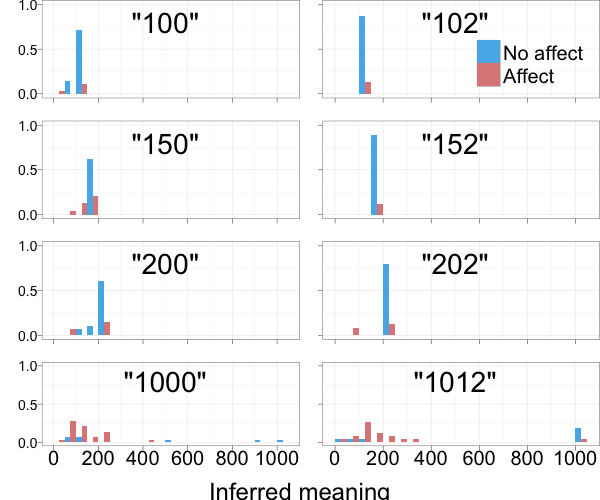
\includegraphics[width=0.65\textwidth]{humans_textbook_all.png}
	\caption{Textbook costs}
\end{figure}
\qquad
\\
% parking
\begin{figure}[h]
	\centering
	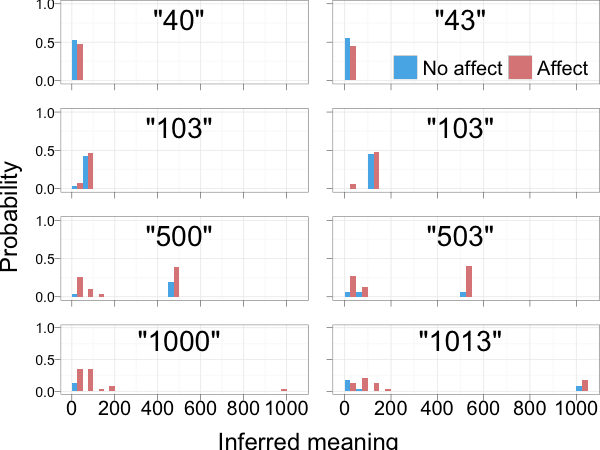
\includegraphics[width=0.65\textwidth]{humans_ticket_all.png}
	\caption{Parking ticket costs}
\end{figure}

% bus
\begin{figure}[t]
	\centering
	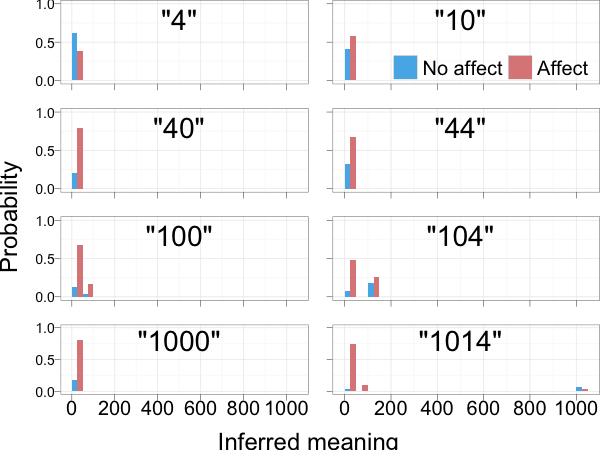
\includegraphics[width=0.65\textwidth]{humans_bus_all.png}
	\caption{Bus wait time}
\end{figure}

% reading
\begin{figure}[b]
	\centering
	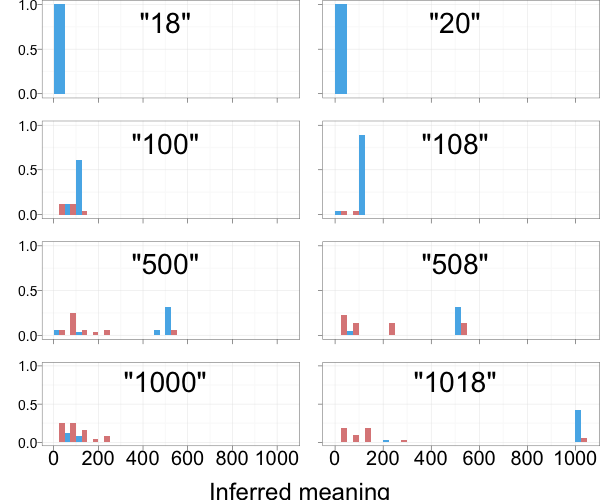
\includegraphics[width=0.65\textwidth]{humans_reading_all.png}
	\caption{Length of reading assignments}
\end{figure}

% weather
\begin{figure}[h]
	\centering
	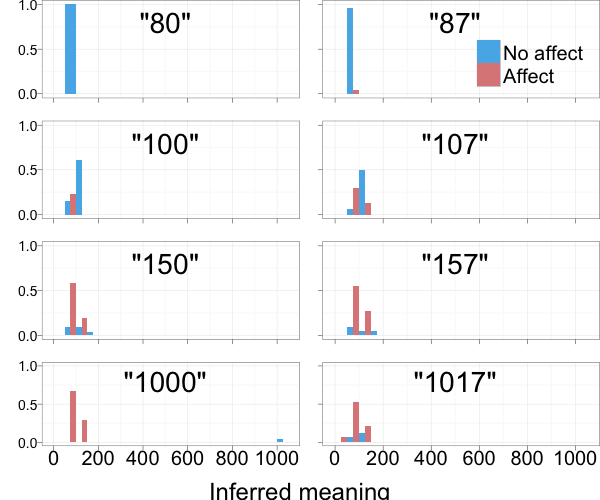
\includegraphics[width=0.65\textwidth]{humans_weather_all.png}
	\caption{Weather temperature}
\end{figure}

\end{document}
